\documentclass[12pt]{article}
\usepackage{latexsym}
\usepackage{amssymb,amsmath}
\usepackage[pdftex]{graphicx}

\topmargin = 0.1in \textwidth=5.7in \textheight=8.6in

\oddsidemargin = 0.2in \evensidemargin = 0.2in

\begin{document}

\begin{center}
COMPUTER SCIENCE 20, SPRING 2014 \\
Homework Problems\\
Author: Tawheed Abdul-Raheem\\
Sets, Relations, Functions, and Countability
\end{center}

\smallskip

\begin{enumerate}
\item Suppose that $A \subseteq B \subseteq C \subseteq D \subseteq E$ and $A \neq C$, $B \neq D$, $C \neq E$. Two of the four statements $A\neq B$, $B \neq C$, $C \neq D$, $D \neq E$ must be true, but there are three acceptable combinations of two. Show which possibilities are valid and why (ex. argue that the truth of $X \neq Y$ and $W \neq Z$ is compatible with the facts for three pairs of the form ($X\neq Y$, $W\neq Z$)).\\

The three acceptable combinations of two are ( $A \neq B$ and $C \neq D$ ) this is true because $B = C$ and $D = E$, the second pair that is acceptable is ($B \neq C$ and $C \neq D$) this is true because $A = B$ and $D = E$, the third acceptablecombination is ($B \neq C$ and $D \neq E$), this is because $A = B$ and $C = D$.

The other three combinations are not acceptable because they happen to contradict our statement. The pairs are ($A \neq B$ and $B  \neq C)$ this means that $C = D$ and $D = E$ which happens to contradict the statement $C \neq E$. Secondly ($A \neq B$ and $D \neq E$, this combination will mean that $C = D$ and $B = C$ which happens to contradict the statement $D \neq B$. Finally the pairs that are not acceptable are ($C \neq D$ and $D \neq E$) this because, for that to be true will mean that $A = B$ and $B = C$ which happens to contradict the statement $A \neq C$

\item Consider $f : A \rightarrow B$, where $A$ and $B$ are finite sets with the same cardinality and $f$ is a total function.  Prove that $f$ is surjective if and only if it is injective and that in this case there exists an inverse function $g : B \rightarrow A$ such that $g \circ f$ is the identity function. \\

To prove that if $f$ is surjective then it is injective, we know that $A$ and $B$ are finite sets with the same cardinality, this means that we have the same number of arrows pointing out of $A$ as we have elements in $B$. For this relationship to be injective it must be that all the elements in $B$ has at most one arrow that maps to it. If we were to have two arrows pointing to one element in $B$, this will mean that the relationship is not injective. Also having two arrows point to one item in $B$ will mean that there is at least one element that does not have an arrow pointing to it. By definition for a relationship to be surjective all the elements in the codomain must have at least one arrow coming to it. Also to prove that if $f$ is injective then it is surjective, by definition of injection all the elements in the codomain must have at most one arrow mapping to it. If we have two arrows mapping onto one item in our codomain this will mean that it is not injective. Now because we know that both sets have the same cardinality and also per our definition of injection this would imply that the relationship is also surjective. Finally due to our one-to-one correspondence (bijection), we can say for $g \circ f$ has an identity because we can't have a correspondence from $g$ to $f$ that has two arrows.

\item Show that for any finite set $S$, $|\mathcal{P}(S)|=2^{|S|}$. (\emph{Hint: use induction on $|S|$.}) \\

\textbf{Base case: } S = 0 \\
    $\mathcal{P}{( S )} = \{ \emptyset \}$ \\
    $|\mathcal{P}{( S )}| = 1$ \\
    $2^{0} = 1$ \\
    \textbf{Inductive hypothesis: } For any set of n elements $|s| = n$, $n \geq 0 $ \\
    $|\mathcal{P}{( S )}| = 2^{|S|} = 2^n$ \\
    $|S| = n + 1$\\
    We need to show that: \\
    $|\mathcal{P}{( S )}| = 2^{|n+1|}= 2^{|n|} \cdot 2^{1} = 2^{|S|} \cdot 2^{1}$ \\
    \textbf{Inductive Step: } We have a set of $n$ elements  
    from this set we can create all the possible different subsets. Now lets say that we added a new 
    element into the set, we take all the subsets, then  make duplicate of every one of them with the new element. In relation to the big set  we still have our old subsets and their duplicates including the new subset. We now have $2^{n}$ old subsets (by the inductive hypothesis) and the same amount of new subsets. That is in total\\
    $2^{n} + 2^{n}$ \\
    $2^{n} \cdot 2^{1}$ \\
    $2^{n+1}$

\item Show that if $A$ and $B$ are countable, then $A \times B$ is countable.\\

    To show that if $A$ and $B$ are countable, then $A \times B$, there are three cases that we are intrested in exploring for the verification that it is indeed true. First is if both sets are finite, by definition we know that sets $A$ and $B$ are finite sets then the cross product of the two sets are also finite therefore it must be countable. 

    The second case is when one of the set is finite and the other is infinite, to prove that this is countable we pair each infite element with our finite set, this association is possible because we know the end of our finite set and also know its cardinality. An example would be to take the first infinite element $\times$ the elements in our finite set. We dont move to the next infinite number until we exhaust all the possible numbers. See below for image. The red line draw shows how the cross product of the two sets was derived.
    \begin{center}
    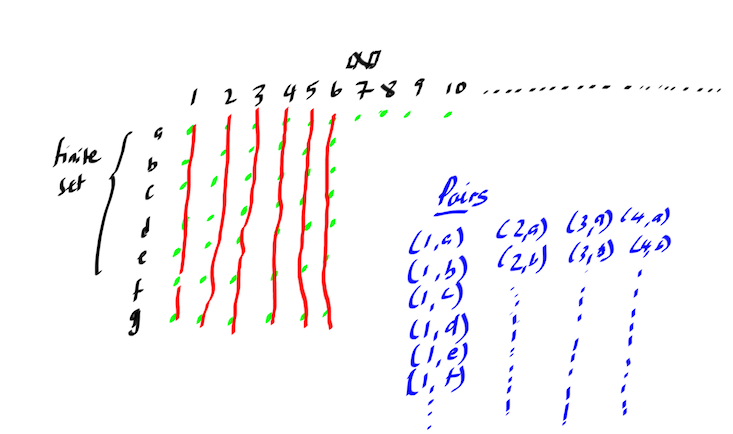
\includegraphics[scale=0.55]{infinity.png}
    \end{center}
    The final case that we need to examine is when both sets are infinite, proving the countablility of an infinite set is a little bit harder than the finite set because it does not have an end and also we wont know when to move to the next pair. The approach we can use is to not try to exhaust all the possible cross products on the first pass through, but rather find them in a diagonal order. See below image of how we can prove the countability of two infinite sets
    \begin{center}
    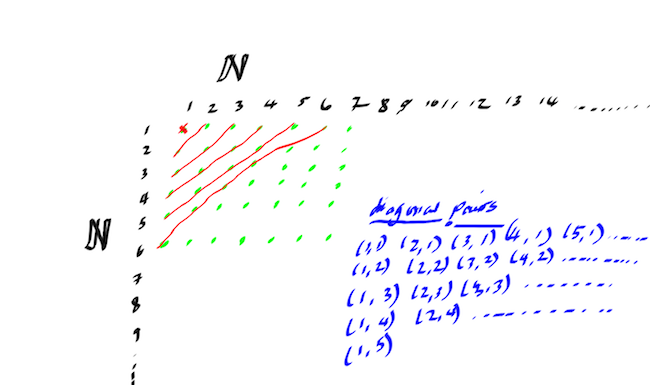
\includegraphics[scale=0.55]{nxn.png}
    \end{center}
\item Show that the set of all functions $f:\{0,1\} \rightarrow \mathbb{N}$ is countable. (\emph{Hint: show that there is a bijection between the set of such functions and the set $\mathbb{N} \times \mathbb{N}$.}) \\

To show that the set of all functions $f:\{0,1\} \rightarrow \mathbb{N}$ is countable, we find all the cross product between our function and the natural numbers. This approach wont lead us to any result as we dont know when our $\mathbb{N}$ ends. So rather than going through an exhaustive list of $\mathbb{N}$ that does not have an end, we can use a diagonal pairing approach where we pair step by step. The idea behind the diagonal pairing is that we get to find the countability of sets by expanding our grounds instead of doing an exhausitive linear pairing that potential does not have an end to it.

\end{enumerate}
\end{document} 
